\section{Contextual Analyzer}
	This section details how scope rules and type rules are checked through the use of a contextual analyzer.
	To use these to check we need a way to visit the abstract syntax tree created with the parser. We have chosen to use 
	the Visitor Design Pattern to traverse the AST received from the parser.
	
	\subsection{The Visitor Pattern}
		The idea behind design pattern is that we send a "Visitor" around the tree structure starting from the top-most node. When a node is 
		visited it lets the visitor know which leaf-nodes it should visit next. \\
		
		\subsubsection*{Small example}
			Here is a small example of how the visitor pattern works using the figure \ref{fig:simpletree}. 
			The visitor is first sent to the node A, from here it is sent to B and C. From C it is sent to D and E.
		
			\begin{figure}
				\centering
				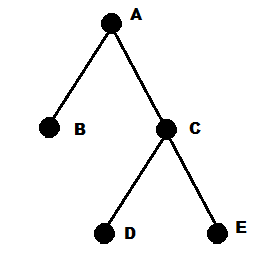
\includegraphics{rapport/6/figures/simpletree}
				\caption{Simple tree} \label{fig:simpletree}
			\end{figure}
			
		\subsubsection{Implementation of the visitor pattern}
			The design pattern was implemented by having a \textit{Visitor} class which includes methods of what to do when a node is visited 
			(e.g. which nodes to visit). Each node in the AST has a Visit method which calls the right Visit methods in the \textit{Visitor} class. \\
	
	\subsection{Identification table}
		For keeping track of the variables or constants defined we use an identification table. The identification table contains entries
		that holds the information of the variable/constant name and the scope level it was defined in.
		
	\subsection{Scope Rules checking}
		Scope rule checking is done by having two methods for opening and closing scope called OpenScope and CloseScope. 
		For keeping track of the scope level we use an integer called {\it level}.
		When the visitor visits a node which requires a scope opening (e.g. RegimentBlock) the OpenScope method is called. 
		This method increases the level variable by 1. After it has visited the required nodes the CloseScope function is called. 
		This removes all the variables and constants defined in this scope level and decreases the level by 1.
	
	\subsection{Type Rules checking}
		When the visitor visits a node where type checking is needed (e.g. RegimentStat), the visitor visits the nodes 
		in need of identification. In each of the visited nodes visit methods the information of the data type is being retrieved 
		from the identification table. The process of finding the data type of variables/constants is called decoration. 
		When the type rules checking is done the AST that is traversed is fully decorated.
		
		